% Generated by Listas/make_statements.py from pratica-lecture-01.md, item 3. Do not edit.
\textbf{Source.} Muñoz-Garcia \& Toro-Gonzalez (2019), \emph{Strategy and Game Theory: Practice Exercises with Answers}, Ch. 1, Exercise 2 ``From Extensive Form to Normal Form Representation-II'', p.~4 {[}PDF 17{]}. Reproduced verbatim (statement only; the book's worked answer follows it).



\begin{quote}

Consider the extensive form game in Fig. 1.3.



\pandocbounded{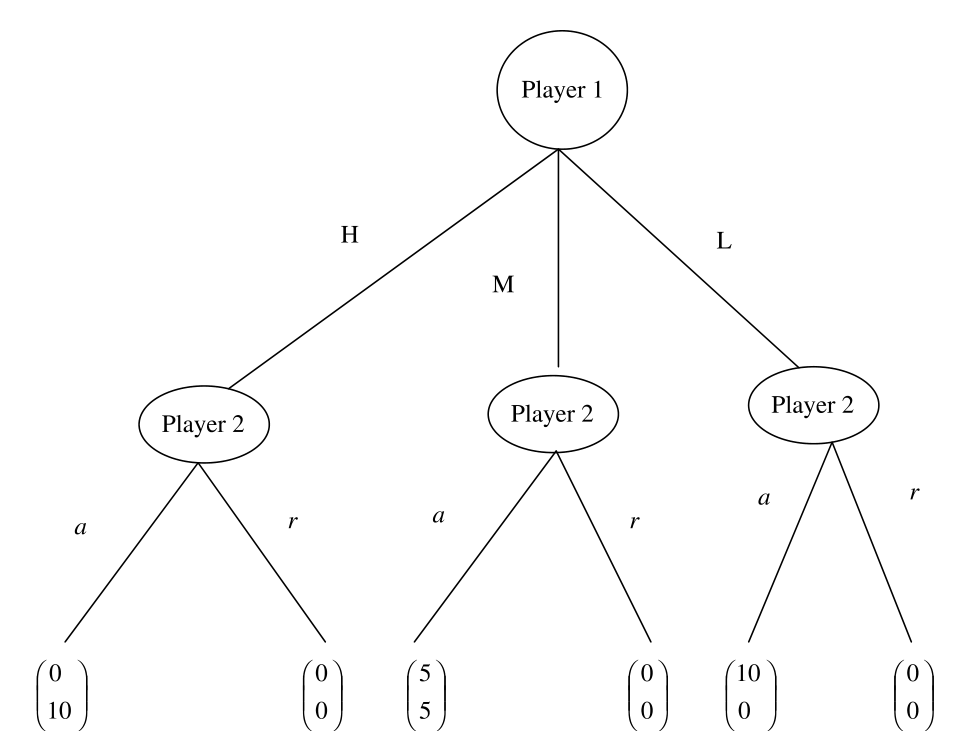
\includegraphics[keepaspectratio,alt={Fig. 1.3 Extensive-form game}]{../figures/munoz-garcia-1-2.png}}



\emph{Fig. 1.3} Extensive-form game



\textbf{Part (a)} Describe player 1's strategy space.



\textbf{Part (b)} Describe player 2's strategy space.



\textbf{Part (c)} Take your results from parts (\emph{a}) and (\emph{b}) and construct a matrix representing the normal form game of this game tree.

\end{quote}

